\documentclass{article}
\usepackage{amsmath}
\usepackage{xcolor}
\usepackage{gensymb}
\usepackage{ragged2e}
\usepackage{graphicx}
\usepackage{gensymb}
\usepackage{mathtools}
\newcommand{\mydet}[1]{\ensuremath{\begin{vmatrix}#1\end{vmatrix}}}
\providecommand{\brak}[1]{\ensuremath{\left(#1\right)}}
\providecommand{\norm}[1]{\left\lVert#1\right\rVert}
\newcommand{\solution}{\noindent \textbf{Solution: }}
\newcommand{\myvec}[1]{\ensuremath{\begin{pmatrix}#1\end{pmatrix}}}
\let\vec\mathbf
\begin{document}
\begin{center}
        \textbf\large{CHAPTER-9 \\ TRIANGLES}
\end{center}
\section{Exercise 11.4}
Question(4).Construct a triangle $XYZ$ in which $\angle{Y}=30^0$,$\angle{Z}=90^0$ and $XY+YZ+ZX=11cm$. \\

\textbf{Solution:}\\
Let $\vec{X}$,$\vec{Y}$ and $\vec{Z}$ are the vertices of the triangle with coordinates.
Given $XY+YZ+ZX=8cm$.So the coordinate of the vertice  $\vec{X}$ is:
\begin{center}
{
$\vec{X} =\myvec{0\\0}$
}
\end{center}
Also given $\angle{Y}=30^0$ and $\angle{Z}=90^0$ so by finding the length of sides we can form a required triangle. \\
 The input parameters for this construction are\\
 \begin{table}[h]
	 \centering
	  \begin{tabular}{|c|c|c|} 
  \hline 
  \textbf{Symbol}&\textbf{Value}&\textbf{Description}\\ 
  \hline 
  $c+a+b$ & 11 & $XY+YZ+ZX$ \\ 
  \hline 
 $\angle{Y}$ & 30$\degree{}$ & $\angle{Y}$ in $\triangle$$ABC$\\ 
  \hline 
        $\angle{Z}$ & 90$\degree{}$ & $\angle{Z}$ in $\triangle$$XYZ$ \\
   
  \hline  
	 $\vec{e}$_1 & $\myvec{ 
   1 \\
   0 \\
   0 
   }$ & Basis vector\\ 
 \hline
 \end{tabular}\\	

	 \caption{Parameters}
	 \label{tab:table1}
 \end{table}\\

 From the given information\\
 \begin{align}
     a+b+c=k\\
     b\cos{Z}+c\cos{Y}-a=0\\
     b\sin{Z}-c\sin{Y}=0
 \end{align}
 Resulting in the matrix equations:\\
 \begin{align}
     \myvec{1 & 1 & 1\\-1 & \cos{Z} & \cos{Y}\\0 & \sin{Z} & -\sin{Y}}\myvec{a\\b\\c}=ke1
 \end{align}
  Substitute the values of k,$\vec{e_1}$,$\angle{Y}$ and $\angle{Z}$\\
  \begin{align}
       \myvec{1 & 1 & 1\\-1 & \cos{90\degree} & \cos{30\degree}\\0 & \sin{90\degree} & -\sin{30\degree}}\myvec{a\\b\\c}= 11\myvec{1 \\ 0 \\ 0 }
  \end{align}
  \begin{align}
      \myvec{1 & 1 & 1\\-1 & 0 & \sqrt{3}/2\\0 & \1 & -1/2}\myvec{a\\b\\c}= 11\myvec{1 \\ 0 \\ 0 }
  \end{align}
  From the above matrix we get the equations as:\\
  \begin{align}
      a+b+c=11\\
      -a+c\sqrt{3}/2=0\\
      b-c/2=0
  \end{align}
  From the equations 8 and 9 we get:\\
  \begin{align}
      a=c\sqrt{3}/2\\
      b=c/2
  \end{align}
  Substitute the above equations in equation 6,we get the value of c:
  \begin{align}
      c=\frac{22}{3+\sqrt{3}}\\
      c=4.65
  \end{align}
  Therefore we get the values of a and b :
  \begin{align}
      a=4.03\\
      b=2.32
  \end{align}
  Therefore the coodinates of the vertices are:
  \begin{align}
      X=\myvec{0\\0}\\
      Z=\myvec{c/2\\0}=\myvec{b\\0}=\myvec{2.32 \\ 0}\\
      Y=\myvec{c/2 \\ c\sqrt{3}/2}=\myvec{b \\ a}=\myvec{2.32 \\ 4.03}
  \end{align}
 Construction:\\
 \begin{figure}[h]
	 \begin{center}
		 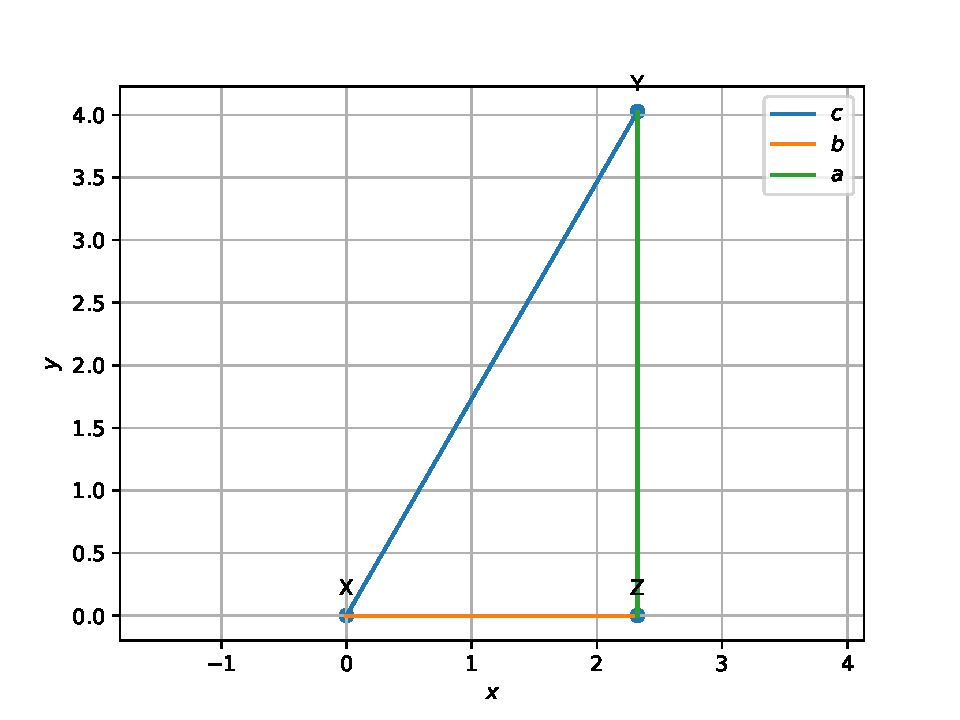
\includegraphics[width=\columnwidth]{code/fig.pdf}
	 \end{center}
	 \caption{Triangle XYZ}
	 \label{fig:Fig1}
 \end{figure}

\end{document}
